%
% File naacl2019.tex
%
%% Based on the style files for ACL 2018 and NAACL 2018, which were
%% Based on the style files for ACL-2015, with some improvements
%%  taken from the NAACL-2016 style
%% Based on the style files for ACL-2014, which were, in turn,
%% based on ACL-2013, ACL-2012, ACL-2011, ACL-2010, ACL-IJCNLP-2009,
%% EACL-2009, IJCNLP-2008...
%% Based on the style files for EACL 2006 by 
%%e.agirre@ehu.es or Sergi.Balari@uab.es
%% and that of ACL 08 by Joakim Nivre and Noah Smith

\documentclass[11pt,a4paper]{article}
\usepackage[hyperref]{naaclhlt2019}
\usepackage{times}
\usepackage{latexsym}

\usepackage{url}

%\aclfinalcopy % Uncomment this line for the final submission
%\def\aclpaperid{***} %  Enter the acl Paper ID here

%\setlength\titlebox{5cm}
% You can expand the titlebox if you need extra space
% to show all the authors. Please do not make the titlebox
% smaller than 5cm (the original size); we will check this
% in the camera-ready version and ask you to change it back.

\newcommand\BibTeX{B{\sc ib}\TeX}

%%%%%neww added commands by writer%%%%%%
\newcommand{\PA}[1]{{\textcolor{blue}{#1}}}
\newcommand{\question}[1]{{\textcolor{orange}{#1}}}

\renewcommand{\labelitemii}{$\diamond$}

\usepackage{amssymb}
\usepackage{amsmath}
\usepackage{amsfonts}
\usepackage{graphicx}
\usepackage[]{algorithm2e}

%%%%%neww added commands by writer%%%%%%

\title{A Navigation Web Search System for Expert Tracking using Deep Reinforcement Learning Approach}

\author{Pegah Alizadeh \\
  Affiliation / Address line 1 \\
  Affiliation / Address line 2 \\
  Affiliation / Address line 3 \\
  {\tt email@domain} \\\And
  Josue Urbina \\
  Affiliation / Address line 1 \\
  Affiliation / Address line 2 \\
  Affiliation / Address line 3 \\
  {\tt email@domain}
  Carl Posthuma \\
  Affiliation / Address line 1 \\
  Affiliation / Address line 2 \\
  Affiliation / Address line 3 \\
  {\tt email@domain} 
  Jorge Garcia \\
  Affiliation / Address line 1 \\
  Affiliation / Address line 2 \\
  Affiliation / Address line 3 \\
  {\tt email@domain} 
  Ivan Meza \\
  Affiliation / Address line 1 \\
  Affiliation / Address line 2 \\
  Affiliation / Address line 3 \\
  {\tt email@domain} 
  Luis Pineda \\
  Affiliation / Address line 1 \\
  Affiliation / Address line 2 \\
  Affiliation / Address line 3 \\
  {\tt email@domain}
  \\}
\date{}

\begin{document}
\maketitle
\begin{abstract}
We present a modification of \textit{Unoporuno} system first introduced by Flores et al. \citep{Flores2012} as an application of deep reinforcement learning and natural language processing methods to the immigration sociology. A manually extracted database containing researcher and experts of central and south America is supported by the sociologists. By receiving a person name from the sociologists database, We propose a method for extracting her organisation names and related activate years over her professional years using deep reinforcement learning approach. We improve the unoporuno system by tracking each person's professional movements instead of just verifying the hers mobility w.r.t her origin place. 
\end{abstract}

\section{Introduction}
Luis Fernandez left his origin country (Argentina) in  $2005$ for doing a PHD in telecommunication. What does he do now? where is he now? where were other universities or organisations that he has worked for so far? for which periods? what are his specialties? In the other words what is his professional track. Sociologists of immigration and particularly those who are interested in ``brain drain" domain requires great deal of time, manual internet search or data source search (such as CVs, personal Web Pages, etc.) to answer such fine-grained examples \cite{Auriol2010,Meyer2006}.

%%%%%%%%%%%
\begin{figure}[!t]
\centering

\includegraphics[scale=0.3]{./images/trajectory.png}
\caption{}
\label{fig:traj}
\end{figure}
%%%%%%%%%

\PA{may be some sate of the art should be added through the following explanation}\\
In this work, we are interested in extracting a trajectory of a given expert including his organisation names and their related years.  For instance, a researcher as ``Luis Fernandez" has a mobile and changeable professional trajectory as figure~\ref{fig:traj} (top graph) while another person (the bottom graph) has a imobile professional trajectory. 

An intuitive approach for tracking any expert professional trajectory contains two parts: querying various research engines with different keywords and extracting name entities (organisation names and years) from the list snippets generated by each query. The main dilemma is that when is the proper moment for generating a new query and which snippets should be selected to extract more informative information w.r.t the expert professional trajectory. According to figure~\ref{fig:naviagte} 

\begin{figure}[!t]
\centering
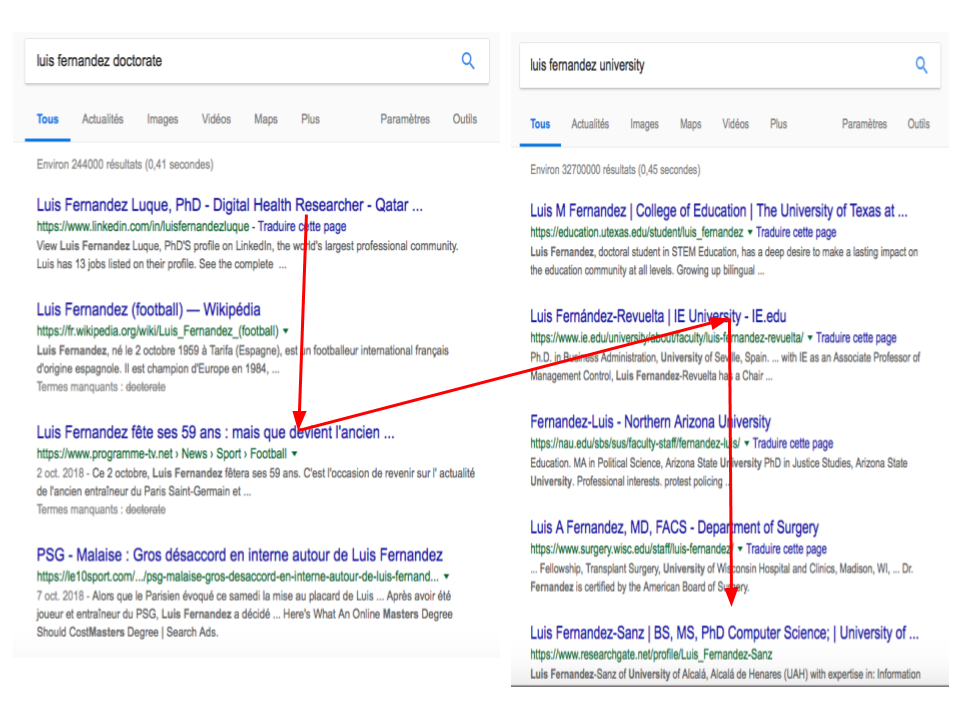
\includegraphics[scale=0.22]{./images/navigate.png}
\caption{\PA{This figure motivates the usage of reinforcement learning in navigating web. But it has two problems: quality and confidential names. Even if I selected a common general Spanish name.}}
\label{fig:naviagte}
\end{figure}

\section{Related Work}

In this section we review the literature of the used \textit{Deep Reinforcement Learning (DRL)} methods for extracting information and introduce a background on application of \textit{Natural Language Processing (NLP)} and DRL methods on sociology of migration application and Web People Search (WPS) tasks. 

\paragraph{Web People Search (\PA{or any similar title reviewing the literature for navigating immigration data base in the web})}

\paragraph{Deep Reinforcement Learning}
In the Reinforcement Learning (RL) environment with a state set $S = s_1, \cdots, s_m$ and a  set of possible actions $A = a_1, \cdots, a_m$, the agent interacts with the environment by selecting an action $a$ in each state $s$ and going to the next state $s'$ until the terminal state condition is satisfied. This process is guided by a function namely \textit{policy} $\pi : S \longrightarrow A$ by interacting the environment. The policy is calculable by assigning a punishment or reward $r(s, a)$ to each selected action $a$ in any state $s$ and maximizing the expected some of rewards \cite{sutton1998}.  

A way of defining the quality of policies is the Q-value function $Q : S \times A \longrightarrow \mathbb{R}$ given by: 
$$Q^{\pi}(s, a) = \mathbb{E}[R_1+ \gamma R_2 + \cdots | s_0 = s, a_0 =a, \pi]$$

which is the expectation of sum of rewards by starting in state $s$ taking action $a$ and following policy $\pi$. Here $\gamma \in (0, 1]$ is a discount factor for future rewards. Considering the Q-value of the \textit{optimal policy} as $Q^*$, then the optimal policy is: $\pi^*(s) = \text{argmax}_a Q^{\pi^*}(s, a) \; \forall  s \in S$.  

Q-learning algorithm \cite{sutton1998} is a model free method for learning the optimal Q-value function. Since Q-value function should be calculated for each sequence of state/actions, computing $Q(s, a)$ for real environments with great number of (or continuous) states or actions  is impractical.  To tackle this problem Mnih et al. \shortcite{mnih2015} introduce the Deep Q-network algorithm for approximating the Q-value function with a non-linear multi layer convolutional neural network.  Given state $s$ and action $a$, the DQN gives $Q(s, a; \theta)$ value where $\theta$ are parameters for the neural network. (\question{If we model the Q-value function as $Q(s, .; \theta)$ where gets sate $s$ and outputs a vector of action values is better in term of calculation time. Our current model is the naive form.})




\section{Framework and Solution}
Using a similar framework as Narasimhan et al. \shortcite{narasimhan2016improving}, we model our web navigator model as a Markov Decision Process (MDP) \cite{puterman1994}. . .

This MDP is defined as a tuple $M(S, A, P, r, \gamma)$ where $S$ is a set of states, $A$ is a set of actions, $P :S\times A  \times S  \longrightarrow [0,1]$ is a transition function where $P(s'|s,a)$ encodes the probability of going to state $s'$ by being in state $s$, and choosing action $a$; $r : S \times A \longrightarrow R$ is a reward function (or penalty, if negative) obtained by choosing action $a$ in state $s$. Each 

blah blah blah
\section{Data}
We test the experiments on (\PA{three?}) different datasets.  The first dataset is a collected dataset including (\PA{how many persons in experiment?})  researchers and experts from central and sound America. A few information such as year, organisation, graduate degree, original country, domain and destination country of each person who left his/her original country for, is supported in the dataset prepared by the sociologists. 

Another dataset is \PA{Jorge dataset?}

Finally we experiment the navigation web system on \PA{shooting dataset with LSTM instead of NN in DQN}
\section{Experiments}

\section{Conclusions}

\section*{Acknowledgments}

\bibliography{naaclhlt2019}
\bibliographystyle{acl_natbib}

\appendix

\section{Appendices}
\label{sec:appendix}


\section{Supplemental Material}
\label{sec:supplemental}

\end{document}
